\documentclass[twocolumn]{aastex62}
\usepackage[latin1]{inputenc}
\usepackage[english]{babel}
\usepackage{amsmath}
\usepackage{amsfonts}
\usepackage{amssymb}
\usepackage{makeidx}
\usepackage{graphicx}
%\usepackage[left=2cm,right=2cm,top=2cm,bottom=2cm]{geometry}
\usepackage{color}
\usepackage{appendix}
\usepackage{multirow}
\usepackage[flushleft]{threeparttable}

\newcommand{\Log}{{\rm Log}}
\newcommand{\Ms}{{\rm M}_\odot}
\newcommand{\Zs}{{\rm Z}_\odot}
\newcommand{\au}{{\rm AU}}
\newcommand{\gw}{{\rm GW}}
\newcommand{\gc}{{\rm GC}}
\newcommand{\kl}{{\rm KL}}
\newcommand{\ibh}{{\rm IMBH}}
\newcommand{\imbh}{{\rm IMBH}}
\newcommand{\inn}{{\rm in}}
\newcommand{\out}{{\rm out}}
\newcommand{\bh}{{\rm BH}}
\newcommand{\bhu}{{\rm BH1}}
\newcommand{\bhd}{{\rm BH2}}
\newcommand{\ARGdf}{\texttt{ARGdf}}
\newcommand{\ARCHAIN}{\texttt{ARCHAIN}}

\graphicspath{{./}{./}}

\received{}
\revised{revised to \today}
\accepted{}

\submitjournal{ApJ (not yet ..)}

\shorttitle{IMRIs in GCs}
\shortauthors{Arca Sedda, M. and Amaro-Seoane, P.}

\begin{document}

\title{Intermediate mass ratio formation in globular clusters: perspectives for LISA sources formation}

\correspondingauthor{Manuel Arca Sedda}
\email{m.arcasedda@gmail.com}

\author{Manuel Arca Sedda and Pau Amaro-Seoane}
\affil{Zentrum f\"{u}r Astronomie der Universit\"{a}t  Heidelberg\\
Astronomisches Rechen-Institut\\
M\"onchhofstrasse 12-14\\
Heidelberg, D-69120, DE}
\affil{...}

\begin{abstract}
We study the formation and evolution of intermediate mass ratio inspirals (IMRIs) triggered by the interactions between stellar black holes and an intermediate black hole (IMBH) inhabiting. We show the probability for an IMRI to form is an increasing function of the IMBH mass, representing a viable channel for the development of gravitational wave sources that can be possibly observed with the future generation of detectors.
\end{abstract}

\keywords{black holes - supermassive black holes - galactic nuclei - gravitational waves}


\section{Introduction}

Intermediate mass black holes, with masses in the range $10^2-10^5\Ms$, might represent the missing link between stellar and supermassive mass black holes. Dense stellar systems, such as globular clusters (GCs), are thought to be ideal factories for IMBH production via formation and collapse of a very massive stars through stellar collisions \citep{zwart02, giersz15, mapelli16} or via multiple interactions and mergers between stars and stellar-mass BHs \citep{giersz15}. Unfortunately, a striking observational evidence for the presence of IMBHs inhabiting GCs is still missing due to the the little dynamical effects that these objects have on their surroundings. Indeed, models suggest that several processes can mimic an IMBH, like anisotropies in the GC kinematical properties \citep{zocchi}, or the presence of a dense cluster of stellar mass BHs that dominate the inner cluster centre \citep{AAG18a,AAG18b,AS16,vandermarel10}. Nevertheless, a few observational IMBHs candidates have been found for Galactic GCs \citep{noyola10,lu13,lanzoni13,kiziltan17} and their mass and influence radius might be possibly connected with the host cluster observational properties \citep{AAG18a}. Due to this, finding an unique way to unravel the presence of IMBHs in GCs represents one of the most interesting challenges in modern astronomy. Beside this, the presence of an IMBH sitting in the centre of a dense cluster represents a scenario particularly appealing from the perspectives of gravitational waves (GW) astronomy. Indeed, a compact remnants orbiting the IMBH can enter a regime where GWs emission dominates, leading to the formation of an intermediate mass-ratio inspiral \citep[IMRI,][]{konstantinidis13,haster16,leigh14}, a class of sources possible audible with the next generation of GW observatories like LISA \citep{seoane07,amaro12,seoane18}

However, in the highly dense regions that characterize star clusters centres, the formation of IMRIs is not a smooth process. Indeed, due to the continuous interactions with stars, an IMRI ``progenitor'', namely a tight IMBH-BH binary, might be subjected to strong perturbation induced, for instance by a passing-by BH. The three-body interaction involving the IMBH and the two BHs can lead to a variety of end states, including the formation of an IMRI, a stellar BH binary, the ejection of one BH, or even both, or the development of a head-on collision. 

Quantifying the branching ratio for IMRIs formation constitute a fundamental step to assess the probability to observe these GW sources with the next generation of space-based detectors like LISA\footnote{\url{https://www.elisascience.org/}} \citep{seoane07}, TianQin \citep{tianqin16} or Taiji \citep{taiji17}.

In this paper, we model the potential formation of an IMRI from the interactions between an IMBH and two stellar mass BHs. To reach the aim, we use $N$-body simulations that take into account in particles' equations of motion both the star cluster gravitational potential and post-Newtonian corrections up to 2.5 order. Varying the IMBH and BHs masses, their orbital configuration, and the host cluster structural properties, we build-up three sets consisting of 2000 models each, which allow us to uncover three possible scenarios for IMRIs formation. 

The paper is organized as follows: in Section \ref{num} we present and summarize the numerical setup used to model the IMBH - BH interaction, in Section \ref{met} we discuss the main properties of the simulations outputs, and the implications for GW astronomy, while Section \ref{res} is devoted to the results summary and conclusions. 


\section{Initial conditions}
\label{met}

In this work, we study IMRIs formation via triple interactions involving an IMBH and two stellar mass BHs that inhabit in the centre of a massive star cluster. 
One of the two BHs is bound to the IMBH, while the second BH orbits around the IMBH-BH binary centre of mass. The triple orbital configuration can be dissected into an inner and an outer binary, as sketched in Figure \ref{fig:f1}. This simple picture is complicated by the fact that the triple cannot be considered as an isolated system, as other cluster members can affect its evolution.

\begin{figure}
    \centering
    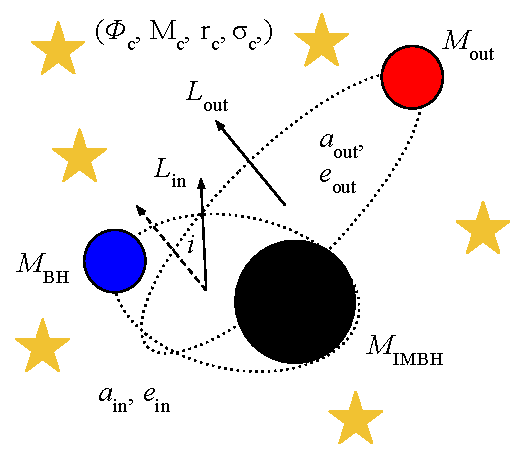
\includegraphics[width=7cm]{triple}
    \caption{Sketch of the IMBH-BH-BH triple configuration.}
    \label{fig:f1}
\end{figure}

Therefore, the phase space that characterises the triple's main properties can be dissected into three groups:
\begin{itemize}
    \item {\bf Inner binary (IMBH+BH)}: depends on the IMBH and BH masses, $M_\ibh$ and $M_\bhu$, the binary semi-major axis $a_\inn$ and its eccentricity $e_\inn$.
    \item {\bf Outer binary (IMBH+BH+BH)}: depends on the third BH mass, $M_\bhd$, semi-major axis $a_\out$, eccentricity $e_\out$.
    \item {\bf Host cluster}: we model the host cluster as a \cite{Deh93} sphere, characterized by total mass, $M_c$, scale radius, $r_c$, and the inner slope of the density profile $\gamma$.
\end{itemize}

In order to unveil the link between IMRIs formation and IMBH properties, we select the IMBH mass among eight different values ${\rm Log}(M_\ibh/\Ms) = 2-2.5-3-3.5-4-4.5-5-5.5$. This range covers typical values of putative IMBH masses forming in stellar systems of various sizes, from young and open clusters, to globular clusters, and up to low-mass nuclear clusters and dwarf galaxies.

Stellar BH masses are selected between $M_{\rm min} = 10\Ms$ and $M_{\rm max} = 30\Ms$, a mass range typical of stellar environments with a metallicity $Z<0.25\Zs$ \citep{belczynski16,spera16}. 
From Figure 5 of \cite{belczynski16}, we find that the BH mass can be connected to the initial star mass via a simple power-law 
\begin{equation}
\left(\frac{m_\bh}{\Ms}\right) = A(Z) \left(\frac{m_*}{\Ms}\right)^{C(Z)} + B(Z),
\end{equation}
with the coefficient depending on the metallicity as summarized in Table \ref{tab:t1}.

Assuming that BH progenitor stars follow initially a standard \cite{kroupa01} initial mass function, $f(m_*) \propto m_*^-s$, we can infer BHs final mass distribution simply as $f(m_\bh)\propto m_\bh^{-s/C(Z)}$. This simple approximation leads to a slope $s/C(Z) = 1.71-1.92$. 

However, we must take into account the fact that during clusters' early evolutionary stages stellar BHs sink into the centre due to mass segregation and start interacting strongly among each other.
As interactions take place, the heaviest BHs are expected to be either kicked out or accreted onto the IMBH seed \citep{giersz15,AAG18a}, potentially causing a strong depletion of BHs especially in the high-end tail of the mass distribution. We assume that the probability for a BH to be ejected or consumed in a merger scales with a weak power of the BH mass, namely $ \propto m_\bh^0.5$. Although quite arbitrary, such choice serves to account for the crucial role played by BHs interactions during the phases that contribute to the IMBH buildup. Given the assumptions above, our models are characterized by a mass function with total slope $\delta_\bh = -2.2$.

\begin{table}
    \centering
    \caption{Stellar - BH mass relation}
    \begin{tabular}{cccc}
        \hline
        \hline
        $Z$ & $A$ & $B$ & $C$ \\
        $\Zs$   &  & &  \\
    \hline    
        $0.005 $& $0.076\pm0.008$ & $3.8\pm0.3$ & $1.35\pm0.02$\\
        $0.25$  & $0.11\pm0.04$   & $0  $       & $1.20\pm0.07$\\
    \hline
    \end{tabular}
    \label{tab:t1}
\end{table}

Inner binary semi-major axis, $a_\inn$, is selected according to a distribution flat in logarithmic values, limited between $10$ and $315$ AU. Same distribution is assumed for the outer binary, but in this case $a_\out$ is chosen in two different ranges, either $a_\out=20-630$ AU or $630-1580$ AU. As detailed below, these ranges characterize two sets of simulations.
The eccentricity is assumed to follow a thermal distribution \citep{jeans19}, $P(e){\rm d}e = 2e{\rm d}e$ for both inner ($e_\inn$) and outer ($e_\out$) binary.

The cosine of the mutual orbital inclination between the inner and outer orbit, $\cos(i)$ is selected randomly between $-1$ and $1$.

The host cluster is assumed to be described by a \cite{Deh93} sphere, characterized by 
total mass $M_c$, scale radius $r_c$ and slope of the density profile $\gamma$.
The cluster length scale $r_c$ is selected randomly between 0.2 and 1.0 pc. For the cluster density slope, we assume a flat distribution with upper limit $\gamma \leq 1$.
To assign clusters' mass we either assume a scaling relation between the IMBH and the cluster mass, $M_\ibh - M_c$, or between the IMBH mass and the cluster velocity dispersion, $M_\ibh-\sigma_c$. 

In the first case, we take advantage of the scaling relations based on numerical models of IMBH formation and observations of putative IMBHs in globular clusters \citep{zwart02,Lutzgendorf13,AS16}. In particular, we adopt the scaling provided by \cite{AS16}, connecting the host cluster mass $M_c$ with the total ''dark'' mass, inhabiting the cluster's centre, comprised of either an IMBH or a sizable population of stellar BHs
\begin{equation}
\Log \left(\frac{M_c}{\Ms}\right) = \alpha \Log \left(\frac{M_\ibh}{\Ms}\right) + \beta.
\label{mcmibh}
\end{equation}
with $\alpha = 0.999 \pm 0.001$ and $\beta = 2.23 \pm 0.009$. 

Similarly to super-massive BHs in galactic nuclei, we can define the IMBH influence radius $R_{\rm inf}$, which delimits the region of space where IMBH dominates dynamics. This quantity can be connected to the cluster structural properties, namely
 \begin{equation}
 R_{\rm inf} = \frac{GM_\ibh}{\sigma_c^2} = \frac{M_\ibh}{M_c}R_{\rm hm},
 \end{equation}
 where we substituted the cluster velocity dispersion $\sigma_c$ with its value calculated at the cluster half-mass radius $R_{\rm hm}$, which in turn can be expressed in terms of the length scale and slope as
\begin{equation}
R_{\rm hm} = r_c(2^{1/(3-\gamma)}-1)^{-1}.
\end{equation} 
Combining the two equations above lead to 
\begin{equation}
R_{\rm inf} = \mu r_c(2^{1/(3-\gamma)}-1)^{-1},
\end{equation}
where $\mu = M_\ibh/M_c = 0.0058$ via Equation \ref{mcmibh}, thus implying that the the IMBH sphere of influence depends only on the cluster scale length and density slope. 

In the second case, instead, we assume that GCs central regions represent a downsized version of galactic nuclei, thus the IMBH mass can be connected to the velocity dispersion inverting the so-called $M_\ibh - \sigma_c$ relation as 
\begin{equation}
     \Log \left(\frac{\sigma_c}{200{\rm km~s}^{-1}}\right) = \frac{1}{\alpha}\left(\left(\frac{\Log M_\ibh}{\Ms}\right) - \beta\right) ,
\end{equation}
with $\alpha = 4.24\pm0.41$ and $\beta=8.12\pm 0.08$ \citep{gultekin09}. Additionally, we associate to the cluster randomly a concentration parameter $c$ between $10.7$ and $131.4$, a range of values typical of dense star clusters characterized by an adimensional potential well $W_0 = 6-9$ \citep{king62}. The cluster mass is then calculated as $M_c = 2\sigma_c^2 c R_c / G$.

We develop three simulations sets, depending on the allowed range for $a_\out$ and the relation assumed to connect the IMBH and host cluster properties. For each set, we run a total of 2000 simulations equally distributed among 8 IMBH mass bins. Therefore, for each value of $M_\ibh$ we gather 250 simulations. The main properties of our runs are summarized in Table \ref{tab:t2}.

Our simulations are performed taking advantage of \ARGdf \citep{ASCD19}, a modified version of \ARCHAIN that implements post-Newtonian dynamics up to order 2.5 and {\it algorithmic regularization} to handle close encounters and strong collisions \citep{mikkola99,mikkola08}. Additionally, \ARGdf allows the user to take into account in particles' equations of motion the gravitational field generated by the host stellary system and a dynamical friction term. Simulations are halted either if one of the two BH merge with the IMBH, if one of the BHs is ejected away of if the simulated time exceeds $t = 10^3 P_{\rm max}$, where $P_{\rm max}$ identifies the maximum between the inner and outer binary orbital period.

\begin{table*}
\begin{center}
\caption{Main properties of our models}
\begin{tabular}{cccccccccccc}
\hline
model   & $f(\Log M_\ibh)$ & $M_\ibh$ & $\delta_\bh$ & $M_\bh$ & $a_\inn$ & $P(e_\inn)$ & $a_\out$ & $P(e_\out)$ &$P(\cos(i))$ &Cluster scaling & $N_{\rm sim}$\\ 
        &             & $\Ms$    &            & $\Ms$   & $\au$    &          & $\au$    &         &  &relation &\\
\hline 
0 & const & $10^2-5\times 10^5$ & $-2.2$ & $10-30$ & $10-315$ & $e^2$ & $20-630$ & $e^2$ & const&$M_\ibh -M_c$ & 2000\\
1 & const & $10^2-5\times 10^5$ & $-2.2$ & $10-30$ & $10-315$ & $e^2$ & $20-630$ & $e^2$ & const&$M_\ibh -\sigma_c$ & 2000\\
2 & const & $10^2-5\times 10^5$ & $-2.2$ & $10-30$ & $10-315$ & $e^2$ & $630-1580$ & $e^2$ &const &$M_\ibh -M_c$ & 2000\\
\hline
\end{tabular}
\end{center}
\label{tab:t2}
\end{table*}



\section{Results}
\label{res}


\subsection{IMRIs formation channels and subsequent evolution}

The evolution of the IMBH-BH-BH triple immersed in the host cluster gravitational field can lead to very different outcomes, as shown in Figure \ref{fig:f3}:
\begin{itemize}
    \item {\bf Disrupted triple} The three-body interaction undergoes a chaotic phases that ultimately lead to the ejection of a stellar BHs, whereas the inner binary either preserves its original components or undergoes a component swap.
    \item {\bf Hierarchical triple.} The triple arranges in a hierarchical configuration, with the outer BHs perturbing secularly the evolution of the inner binary. In this case, the inner binary can develop Kozai-Lidov oscillations \citep{kozai62,lidov62} that can trigger its eccentricity to grow to values close to unity. 
    \item {\bf Unstable triple.} The inner and outer binary are in an unstable configuration, whose evolution is mostly dominated by chaos.
\end{itemize}

\begin{figure*}
    \centering
    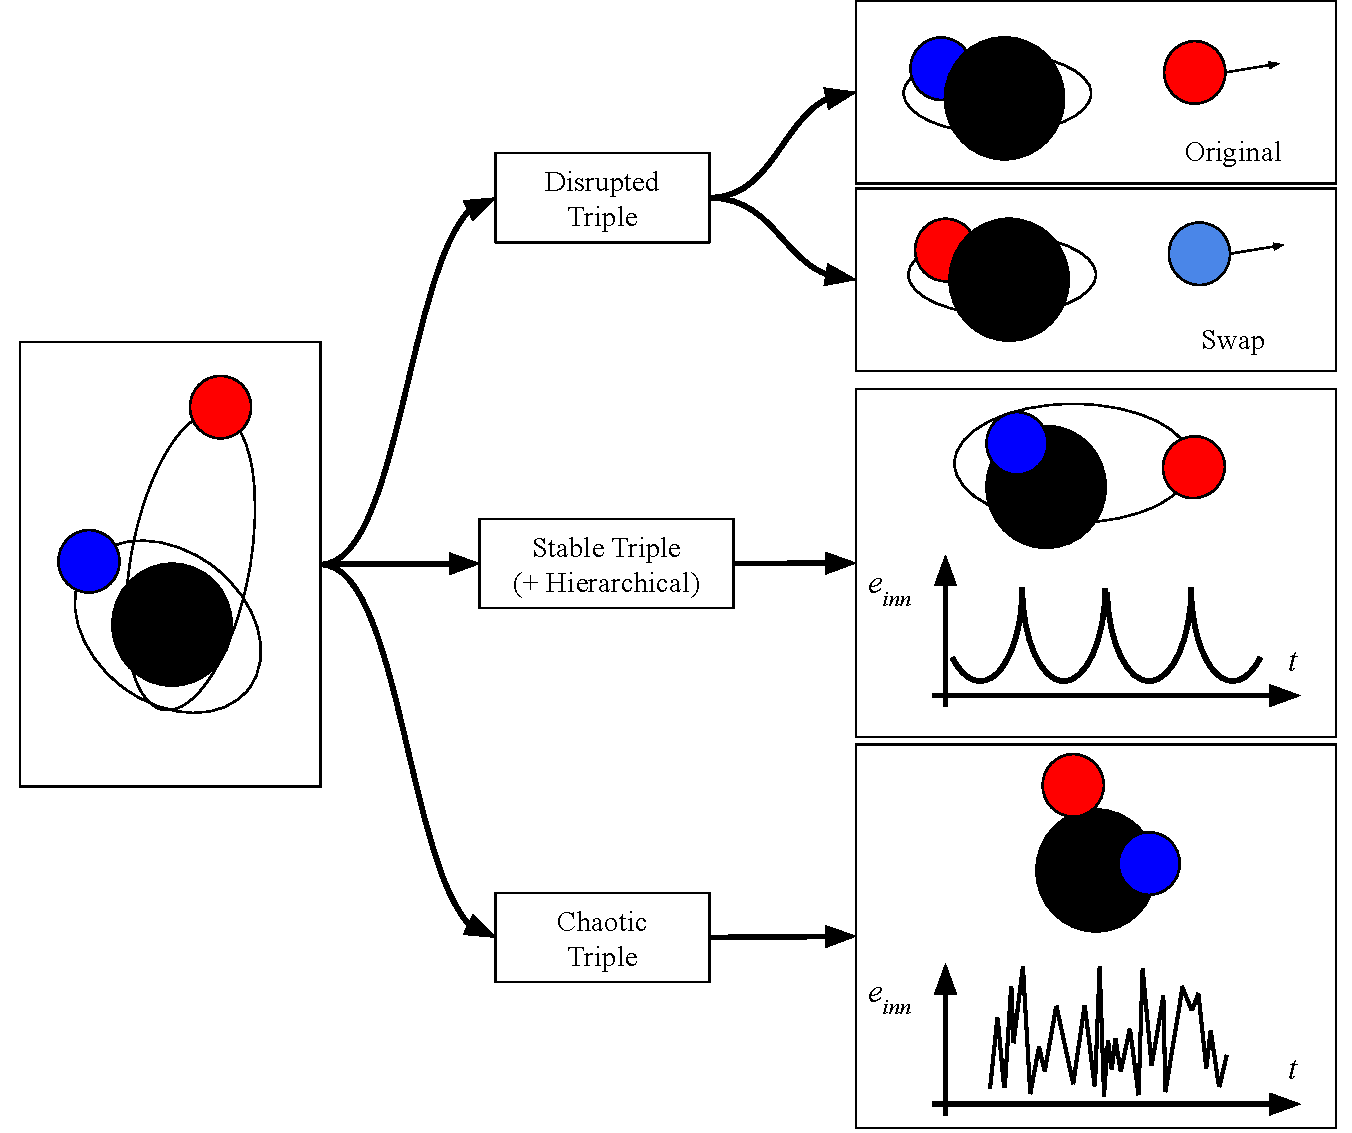
\includegraphics[width=16cm]{Sketch_IMRI}
    \caption{Schematic view of IMBH-BH-BH triple evolution.}
    \label{fig:f3}
\end{figure*}

In case of BH ejection, the evolution of remaining IMBH-BH will be due to the sum of two contributes, namely energy removal from binary-single interactions and GW emission. If the IMBH-BH entered the IMRI phase, binary-single interactions are expected to play little to no effect on its evolution \citep{seoane18}. In this case, the IMRI will continuously shrink emitting GW until coalescence, which takes place on a timescale \citep{peters64}
\begin{align}
t_\gw =&  \displaystyle \frac{5}{256}\frac{c^5 a_\inn^4 (1-e_\inn^2)^{7/2}}{G^3M_\ibh M_\bh(M_\ibh+M_\bh)} = \nonumber \\
       & 10^6{\rm ~yr}\left(\frac{a_\inn}{0.1\au}\right)^4\left(1-e_\inn^2\right)^{7/2}\times \nonumber \\ 
       & \times \left(\frac{10^3\Ms}{M_\ibh}\right) \left(\frac{30\Ms}{M_\bh}\right)\left(\frac{1030\Ms}{M_\ibh+M_\bh}\right).
\label{peters}
\end{align}

We note that for circular IMBH-BH binary in our model ($a_\inn=10\au$) the corresponding merger timescale is $t_\gw \sim 10^{14}$ yr, thus implying that some external perturbation is needed to trigger IMRI formation within a Hubble time.

In the second case, the triple arranges in a hierarchical configuration, whose evolution is dominated by secular perturbations. This mechanism, known as Kozai-Lidov \citep{kozai62,lidov62}, can induce periodic oscillations in the mutual inclination and the inner binary eccentricity. A parameter widely used to discern hierarchical triples is defined as \citep{Lithwick11,naoz11}
\begin{equation}
\epsilon_\kl = \frac{M_\imbh - m_\bh }{M_\imbh + m_\bh} \frac{a_{\inn}}{a_{\out}}\frac{e_{\out}}{(1-e_{\out}^2)},
\end{equation}
being the triple hierarchical if $|\epsilon| > 0.01$.

In this configuration, the eccentricity can increase up to values close to unity \citep{naoz11,naoz16}, leading the inner binary to continuously lose energy via bursts of GWs emitted at each pericentral passage. Therefore, the periodic eccentricity increase can drive the inner binary into the GW emission-dominated regime and trigger the formation of the IMRI. Kozai-Lidov oscillations cause a reduction of the merging timescale \citep[see for instance]{antonini12}
\begin{equation}
    t_{\rm gwKL} = \frac{t_\gw}{\sqrt{1-e_{\rm max}^2}},
\label{kozai}
\end{equation}
being $e_{\rm max}$ the maximum eccentricity achieved by the inner binary. 

In the case of an unstable triple, the inner and outer binaries have similar orbital properties and dynamics is mostly dominated by chaotic interactions. According to the \cite{mardling01} criterion, a triple is unstable if
\begin{equation}
    \frac{a_\out}{a_\inn} < \frac{2.8}{1-e_\out}\left(1-\frac{0.3i}{\pi}\right)\left[\frac{(1+q_\out)(1+e_\out}{\sqrt{1-e_\out}}\right]^{2/5}, 
\end{equation}
being $q_\out = m_\out/(m_\imbh + m_\bh)$.

In our models, we calculate $\epsilon_\kl$ and $a_\out/a_\inn$ at the end of the simulations, in order to identify to which category a triple belongs. The merger time for the inner binary is calculated through Equation \ref{peters} for models categorized as ``Disrupted'' or ``Unstable'', whereas we use Equation \ref{kozai} for those identified as ``Hierarchical''. 

\subsection{IMRIs properties}

We mark as IMRI candidates all IMBH-BH that, by the end of the simulations, have a merger time below 13 Gyr. 

We find quite similar results in both SET0 and SET1, thus implying that both the host cluster mass does not change significantly from one method to the other, and that the external potential has a little effect on the triple evolution. The latter is due to the fact that we are looking in the immediate cluster centre vicinity, where dynamics is dominated by the IMBH.

In SET0, an IMRI develop in $212$ cases out of 2000, i.e. $f_{\rm mer} = 10.6\%$ of formation probability. Concerning the formation channel, $8\%$ of IMRIs formed from Disrupted, $66.5\%$ from Hierarchical, and $25.5\%$ from Unstable . Similarly, in SET1 we find $268$ IMRIs ($13.4\%$), $4.9\%$ of them formed from Disrupted, $67.9\%$ from Hierarchical triples, and $27.2\%$ from Unstable. All IMRIs formation probability for different channels are summarized in Table \ref{tab:t3}.

\begin{table}
    \centering
    \caption{IMRIs formation probability}
    \begin{tabular}{cccccc}
        \hline
        \hline 
        model& $f_{\rm mer}$ & $f_{\rm mer,D}$ & $f_{\rm mer,H}$ & $f_{\rm mer,U}$\\
             & $\%$& $\%$& $\%$& $\%$\\
        \hline
        SET0 & $10.6$ & $8.0$ & $66.5$ & $25.5$ \\
        SET1 & $13.4$ & $4.9$ & $67.9$ & $27.2$ \\
        \hline
    \end{tabular}
    \label{tab:t3}
\end{table}


Figure \ref{fig:f4} shows a comparison between the initial and final distribution of IMRI candidates' semi-major axis and eccentricity. We stress that both $a_\inn$ and $e_\inn$ are calculated from the last snapshot, thus they do not necessarily represent the binary orbital parameters promptly before the mergers. We postpone the discussion on the last stages of the IMRIs evolution to the next section.

The top panel shows clearly that the semi-major axis distribution of merging binaries differs significantly from the initial values, which is nearly uniform in the logarithms by assumption. The final distribution shows a peak at $\sim 10\au$, with a low-end extending down to $\lesssim 0.1 \au$. The eccentricity distribution, which is shown in the bottom panel, highlights that merging binaries tend to have a distribution steeper than the initial, thus implying that merger candidates are characterised by high eccentricities. Note that these distribution does not differentiate models with a different IMBH mass. 

\begin{figure}
\centering
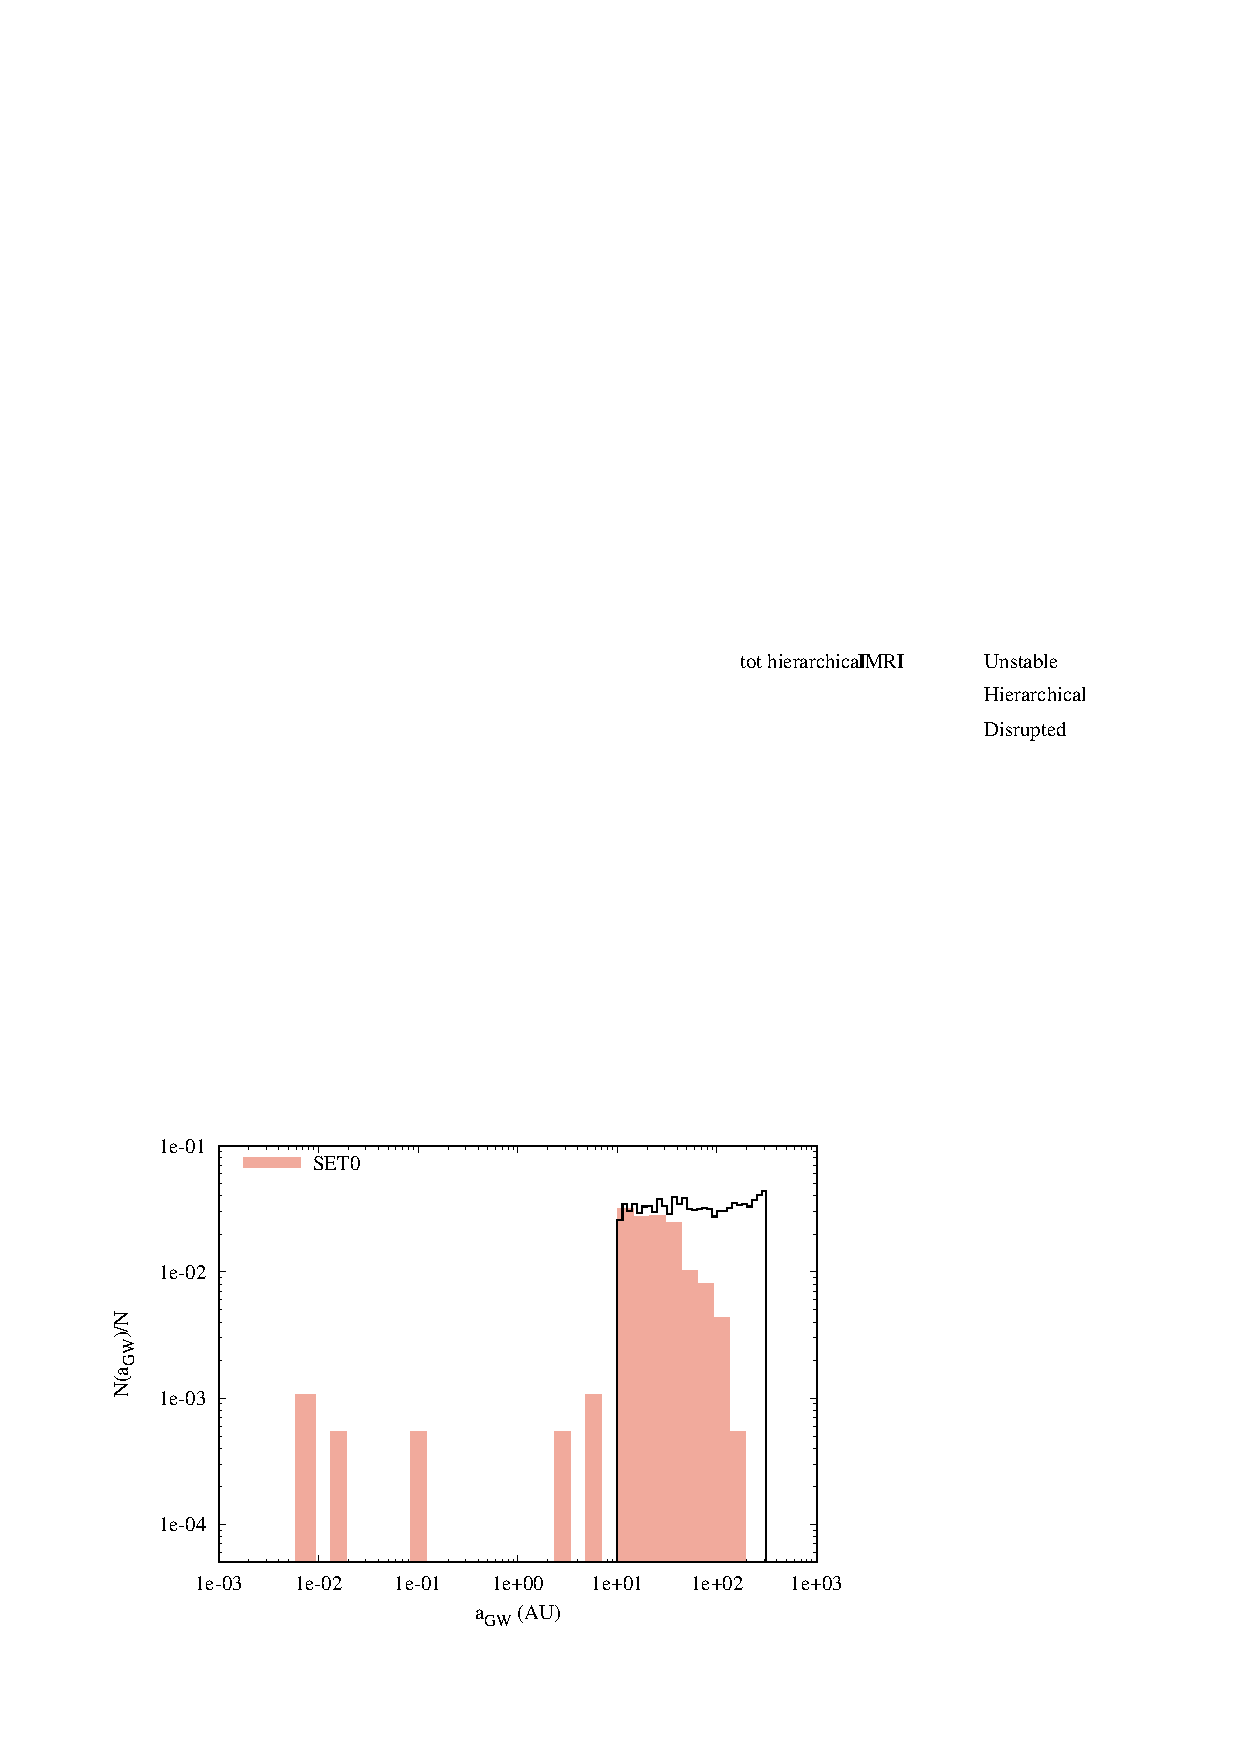
\includegraphics[width=8cm]{semiaxis}\\
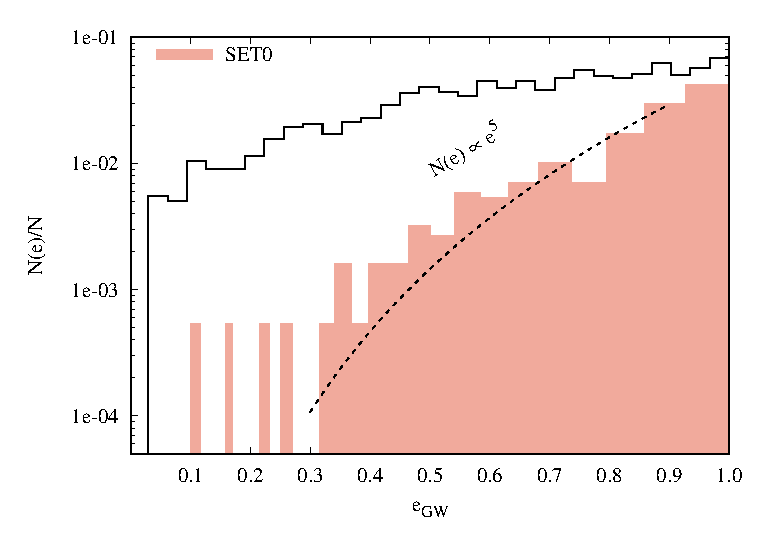
\includegraphics[width=8cm]{ecce}
\caption{Top panel: semi-major axis distribution for the inner binary. The black steps refer to initial values for all the simulations performed, while the red filled steps refer only to merger binaries and final values. Bottom panel: the same as in top panel, but for the inner binary eccentricity.}
\label{fig:f4}
\end{figure}

\subsection{The role of the IMBH mass}

To explore the dependence between IMRI candidates eccentricity at formation and IMBH mass, we take the eccentricity directly from the last snapshot for models targeted as ``Disrupted'' and ``Unstable'', while for ``Hierarchical'' we record the maximum eccentricity. We then calculate the mean eccentricity value $\langle e_\gw\rangle$  in different mass bins, making the same for the subset of IMRI candidates, as shown in Figure \ref{fig:f4}. In general, it seems that, regardless of the set, IMRI candidates with masses below $5\times10^3\Ms$ have, on average, $\langle e_\gw\rangle$ larger compared to the whole simulations sample, while this trend reverses for heavier IMRIs. 

The average eccentricity increases in the $10^2-5\times10^3\Ms$ mass range, peaking at around $500-1000\Ms$, and than decreases rapidly at increasing the IMBH mass.This implies that the evolution of the inner binary leads the eccentricity to achieve larger values in correspondence of lighter IMBHs. 

We find that IMBHs with masses typical of star clusters $10^3<M_\ibh/\Ms<10^4$ are expected to form, on average, extremely eccentric IMRIs, while the eccentricity at formation attains more moderate values at IMBH masses typical of low-mass dwarf galaxies and nuclear clusters.

While affecting the eccentricity, the IMBH mass does not have a significant effect on the companion BH mass. Indeed, IMRIs light component masses follows the assumed BH mass distribution. 

\begin{figure}
\centering
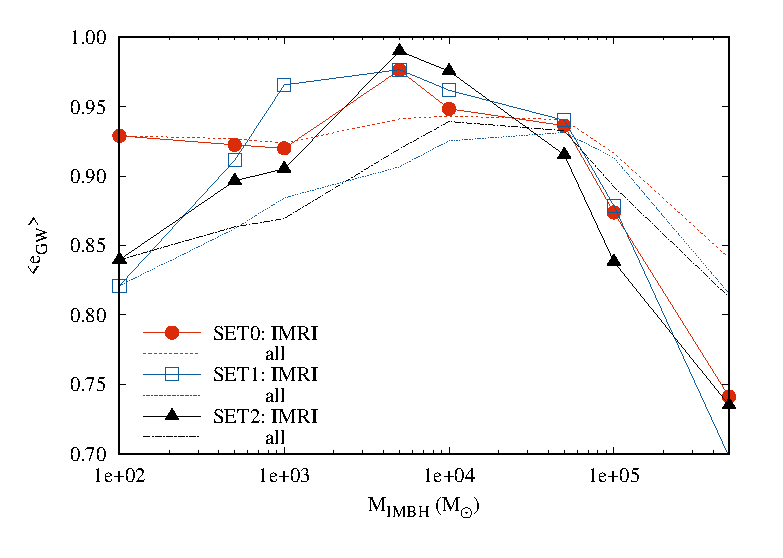
\includegraphics[width=8cm]{average_ecc_sets}\\
\caption{The average eccentricity ($\langle e_{\rm mer}\rangle$), calculated at the end of simulaitons in different IMBH mass bins, as a function of the IMBH mass and for different sets. We show the IMRIs average eccentricity SET0 (filled red points), SET1 (open blue squares), and SET2 (filled black points). The total average value is also marked for SET0 (dashed red line), SET1 (dotted blue line), and SET2 (dot-dashed black line). }
\label{fig:f5}
\end{figure}

In order to uncover what is the role played by the IMBH in determining IMRIs formation, we calculate the 
percentage of IMRIs formed in different mass bins. This quantity, namely $f_{\rm mer}$, represents {\it de facto} IMRIs formation probability. We find that $f_{\rm mer}$ follows quite a precise trend, regardless of the set, thus in what follows we focus on SET0 only, for clarity's sake. Figure \ref{fig:f5} shows the $f_{\rm mer}-M_\ibh$ relation. We differentiate between IMRIs forming in disrupted triples, in a hierarchical or unstable configuration. 
Our results suggest that an IMBH-BH-BH has a $10\%$ of probability to arrange in a hierarchical configuration, regardless of the IMBH mass or the GW timescale. IMRIs formation probability, instead, increases weakly with IMBH mass, increasing from $\sim 2\%$ for $M_\ibh \simeq 10^2$ to up to $15\%$ for heavy IMBH, $M_\ibh>10^5\Ms$.

At IMBH mass values below $10^4\Ms$, we find that Hierarchical and Unstable systems contribute equally to the whole IMRI population, while at larger IMBH masses the majority of IMRIs is comprised of Unstable triples. IMRIs forming out of Disrupted triples give little contribution to the population, being their formation probability only $0.5-1\%$.

In the IMBH mass range $M_\ibh>10^3\Ms$, the IMRIs formation probability is well described by a simple powerlaw
\begin{equation}
f_{\rm mer} = \alpha \left(\frac{M_\ibh}{10^2\Ms}\right)^\beta,
\label{fmerg}
\end{equation}  
with $\alpha = (7\pm2)\times 10^{-3}$ and $\beta = 0.45\pm0.03$. 

\begin{figure}
    \centering
    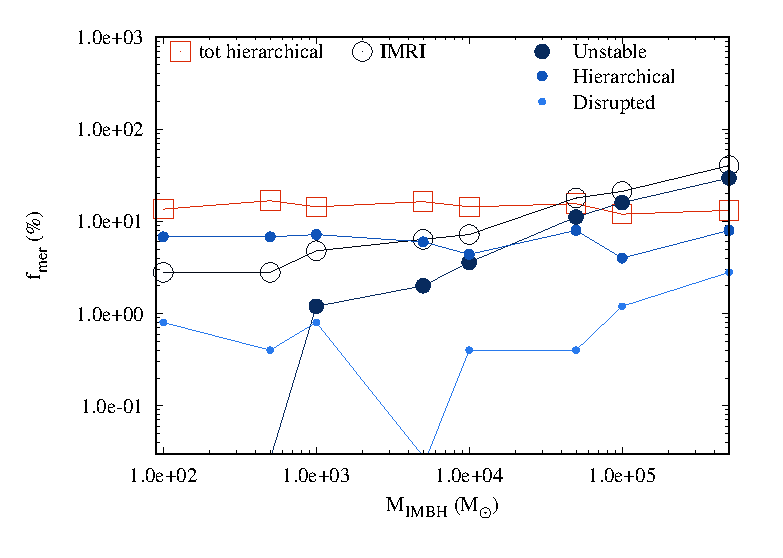
\includegraphics[width=\columnwidth]{mergers.eps}
    \caption{Percentage for IMRIs formation as a function of IMBH mass. Red open squares shows all the models that are hierarchical at the end of the simulation. Open dark blue circles identify IMRIs. From larger to smaller circles, blue filled circles represent IMRIs formed from unstable, hierarchical, and disrupted triples.}
    \label{fig:f5}
\end{figure}

Our simulations suggest that whenever a three-body encounter occurs in a GC containing a $10^4\Ms$ IMBH, there is a $\sim 10\%$ of the probability for IMRIs formation and the eccentricity at formation is of the order of 0.95. 

\subsection{IMRIs merger rate}

{\bf Previous studies based on full consistent N-body simulations of star clusters containing IMBHs with various masses and general properties  \citep{konstantinidis13,haster16,leigh14, macleod16} have shown that binary formation involving an IMBH takes place at a rate of $R_{\rm bin} \sim 10^{-7}$ yr. Assuming typical ages for globular-like star clusters of $t_{\rm age}\sim 10^{10}$ yr and assuming that IMBH buildup occurs in the clusters early lifetime ($\lesssim 1$ Gyr), we can use the merger probability fitting function depicted in Equation \ref{fmerg} to infer IMRIs merger rate per typical cluster
\begin{equation}
    \Gamma(M_\ibh) = R_{\rm bin}t_{\rm age}f_{\rm mer} \sim 0.7\left(\frac{M_{\ibh}}{10^2\Ms}\right)^{0.45},
\end{equation}
ranging from $\Gamma_{\rm IMRI} = 7-50$ yr$^{-1}$ for $M_\ibh = 10^2-10^4\Ms$, respectively.

To put such a quantity in the context of MW-like galaxies, we need to make assumptions on the IMBH putative mass function. As recently suggested by Arca Sedda et al (in prep.), out of the 151 Galactic GCs currently known, around 35 might be harbouring, at present time, an IMBH with mass in the range $10^3-10^4\Ms$. They find that the mass distribution of these putative IMBHs can be described by a Maxwellian in the form 
\begin{equation}
    f(x_\ibh) = \frac{a}{\sigma\sqrt(2\pi)}\exp{\left(-\frac{\left(x_\ibh - \mu\right)^2}{ (2\sigma^2)}\right)},
\end{equation}
with $x_\ibh\equiv \Log M_\ibh$, and $a=0.14\pm0.3$ , $\mu = 4.01\pm0.09$ and $\sigma = 0.4\pm0.1 $.

Combining equations above, we can define a IMRI merger rate for MW-like galaxies as
\begin{equation}
    \Gamma_{\rm MW} = f_\ibh N_\gc \int \Gamma(M_\ibh) f(x_\ibh) {\rm d}M_\ibh,
\end{equation}
where $f_\ibh N_\gc$ is the number of GCs containing an IMBH. This equation has analytical solution
which has analytical solution
\begin{align}
 \frac{\Gamma_{\rm MW} (x_\ibh)}{f_\ibh N_\gc} =&   \frac{a}{2} (A + B\mu) {\rm erf}\left(\frac{x_\ibh-\mu}{\sigma\sqrt{2\pi}} \right) + \nonumber\\
                                & - \frac{a}{\sqrt(2\pi)}B \sigma \exp{\left(\frac{-\left(x_\ibh-\mu\right)^2}{2\sigma^2}\right)},
\end{align}
 the coefficients $A = \alpha -\beta \Log(100)$ and $B \equiv \beta$ are conveniently manipulated from Equation \ref{fmerg}.

Assuming a typical IMBH population spanning the mass range $10^2-10^4\Ms$, a number of GCs $N_\gc = 151$, a fraction $f_\ibh \simeq 35/151$ of GCs hosting an IMBH we can infer the MW-IMRI rate 
\begin{equation}
\Gamma_{\rm MW,IMRI} \simeq 4\times 10^{-3} {\rm MW}^{-1} {\rm yr}^{-1}
\end{equation}



}

\subsection{Serendipitous formation of stellar BH binaries around an IMBH}

Among all the runs performed, we find two interesting cases, namely s151 and s400, in which the stellar mass BHs are initially sufficiently close to form a tight binary. In both cases, the IMBH mass is relatively small $M_{\ibh} = 100\Ms$, and the inner binary is comprised of the other two, stellar-mass, BHs. It is not surprising that a BH-BH pair forms in a model with low-mass IMBH, due to the lower velocity dispersion and the larger tidal radius needed for the binary to form without being ripped apart from the IMBH. In both cases, the BH-BH binary undergoes Kozai-Lidov oscillations, which periodically induce an increase in the binary eccentricity and the mutual inclination.

In model s400, the amplitude of the oscillation is minimal, the mutual inclination ranges between $i = 126-130^\circ$, while the eccentricity varies in the range $e = 0.882-0.904$. Although the KL effect is not very efficient in affecting the BH-BH evolution, the binary is sufficiently tight to have a short merger timescale, being $t_{\rm gw} \simeq 3\times 10^7$ yr.

In model s151, instead, the Kozai-Lidov effect is more effective, leading the inclination to vary strongly in the range $\sim 40-90^\circ$ and the eccentricity to rise up to $e = 0.99$. The time evolution of both $e$ and $i$ is shown in Figure \ref{F9}, together with the associated merger time-scale. 
In this particular simulation, the reduction of the merger time related to the episodic GW emission as described in Equation \ref{kozai}, trigger the BH binary coalesce in a time $5600$ times smaller than the time needed for the same binary to merge in isolation.

In both the cases that we find, the IMBH mass is $M_\ibh=100\Ms$. Heavier IMBHs would make BH-BH pairing much harder, because of the higher velocity dispersion and the larger gravitational influence. Having 250 simulations with $M_\ibh=100\Ms$ in each set, we can infer BH-BH formation probability as $P_{\rm bhb} = 0.8\%$.

\begin{figure}
\centering 
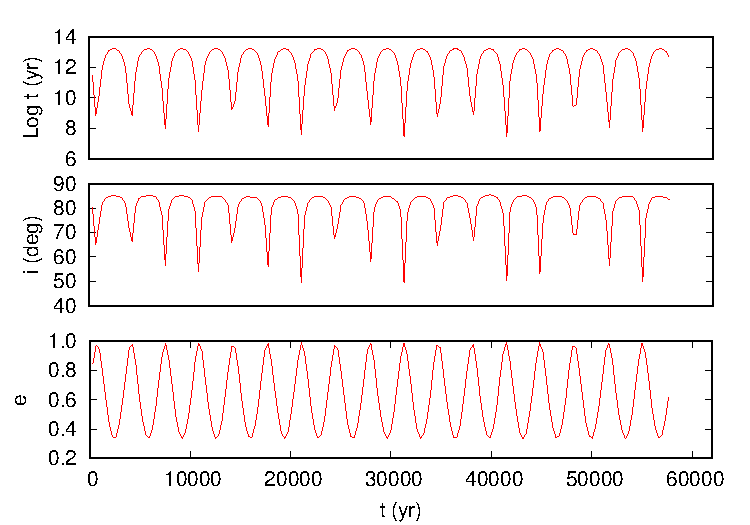
\includegraphics[width=8cm]{kozai_151}
\caption{Top panel: time evolution of the merger timescale for model number 151, in which two BHs pair together while the IMBH acts as a perturber. Central panel: mutual inclination as a function of time for the BH-BH pair in simulation number 151. Bottom panel: ecentricity as a function of time for the BH-BH pair in simulation number 151.}
\label{F9}
\end{figure}

\section{Gravitational waves}

In this section we investigate the properties of IMRIs formed in our model from the perspective of GW emission. To perform our study, we take from the last snapshot of all the simulations the inner binary semi-major axis and either the maximum eccentricity, if the triple is marked as ``Hierarchical'', or the actual eccentricity, if the triple is marked as ``Disrupted'' or ``Unstable''.

In the following, we indicate semi-major axis and eccentricity with $a$ and $e$, respectively, while the IMRI mass is labelled with $M_{\rm bin}$.

As long as the binary preserve a residual eccentricity, the GW signal is audible in a range of frequency, rather than being monochromatic. The peak frequency can be approximated as \citep{wen03, antonini12}
\begin{equation}
f_\gw = \frac{1}{\pi}\sqrt{\frac{GM_{\rm bin}}{a^3}}\frac{\left(1+e\right)^{1.1954}}{\left(1-e^2\right)^{3/2}},
\end{equation}  
being $M_{\rm bin}$ the merging binary total mass. Using this definition, we show in Figure \ref{F10} how the peak frequency and eccentricity vary for mergers in our models. In order to understand whether these sources can be audible to GW observatories, we superpose our calculations to the observational windows of the Laser Interferometer Space Antenna \citep[LISA\footnote{\url{https://www.elisascience.org/}},][]{amaro12}, the Deciherz Gravitational-Wave Observatory \citep[DECIGO\footnote{\url{http://tamago.mtk.nao.ac.jp/spacetime/decigo_e.html}},][]{seto01}, and the Einstein Telescope \citep[ET\footnote{\url{http://www.et-gw.eu/}},][]{punturo10}. 

\begin{figure}
\centering
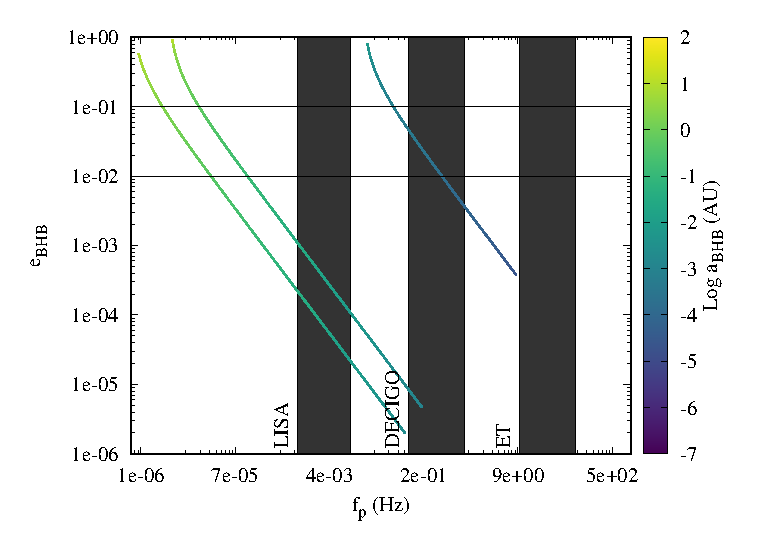
\includegraphics[width=8cm]{freq_evo}\\
\caption{Frequency (x-axis) and eccentricity (y-axis) evolution for merging binaries in our models. The color coding identifies the semi-major axis evolution. Black boxes are a coarse representation of observational windows for LISA, DECIGO and the Einstein Telescope. The horizontal lines mark two values of the eccentricity, namely $e=0.01-0.1$.}
\label{F10}
\end{figure}

We find that more than $95\%$ of the sources in both models transit into the $5\times 10^{-4} - 5\times 10^{-3}$ Hz band, where LISA is sensitive. Approximately $10\%$ instead are characterized by GW emission in DHz regime, being potentially observed with LIGO and, in the future, with DECIGO and ET.
The numbers of sources appearing in different bands are summarized in Table \ref{tab:t4}
 
 \begin{table*}
     \centering
     \caption{IMRI frequency bands}
     \begin{tabular}{ccccccc}
        \hline
        \hline
        model & IMRI - total number & $N_{\rm mHz}$ & $N_{\rm cHz}$ & $N_{\rm dHz}$ & $N_{\rm Hz}$ & $N_{\rm DHz}$ \\ 
              &                     &$0.5-5$ mHz    & $ 0.5-5$ cHz  &  $0.5-5$ dHz & $0.5-10$ Hz & $>1$ DHz \\
        \hline
        SET0 & $211$ & $204$ &  $207$ & $120$ & $46$ & $22$   \\
        SET1 & $268$ & $256$ &  $259$ & $144$ & $56$ & $28$   \\
        \hline
     \end{tabular}
     \label{tab:t4}
 \end{table*}
 
 
It is interesting to note that a handful of sources could have a non-negligible eccentricity both in the LISA and DECIGO observational band, while at larger frequencies the binaries are already completely circular. In order to better highlight the probability for low-frequency detectors to observe eccentric IMRIs, we show in Figure \ref{F11} the eccentricity distribution of sources entering the mHz and Hz frequency bands. We find that only $10\%$ of sources have high eccentricity in the LISA band, while for DECIGO this quantity is slightly smaller ($\sim 7\%$).
 
\begin{figure}
\centering
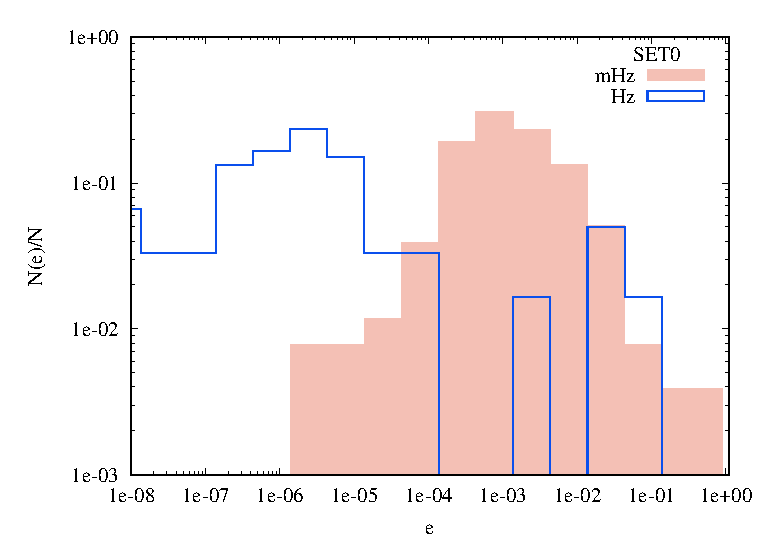
\includegraphics[width=8cm]{mergers_eccen}\\
\caption{Eccentricity distribution for IMRIs in our models. The eccentricity is calculated at the moment in which a source cross the mHz (red filled steps) or Hz frequency band (black steps).}
\label{F11}
\end{figure}

In order to infer whether these sources might be audible to GW observatories, we calculated the strain following \cite{kocsis12} for all the frequencies containing the $95\%$ of the emitted power. We assume a luminosity distance $D_L = 463$ Mpc (redshift $z=0.1$), and a 5 yr observation time. Figure \ref{F12} shows the evolution of the strain-frequency evolution for two different mergers, altogether with the eccentricity decrease due to GW circularization. One merger refers to an IMRI with total mass $M_H$

For the sake of visibility, we only show the strain associated to the dominant frequency. In the two models shown in the plot, the mergers outshine in the LISA band, where they spend most of their life, and slowly shift toward higher frequency, merging inside the LIGO observational band. These sources are of extreme interest since they can be used to further constrain and test the General Relativity theory, as their evolution can be monitored in both the low- and high-frequency regime. 

\begin{figure}
\centering
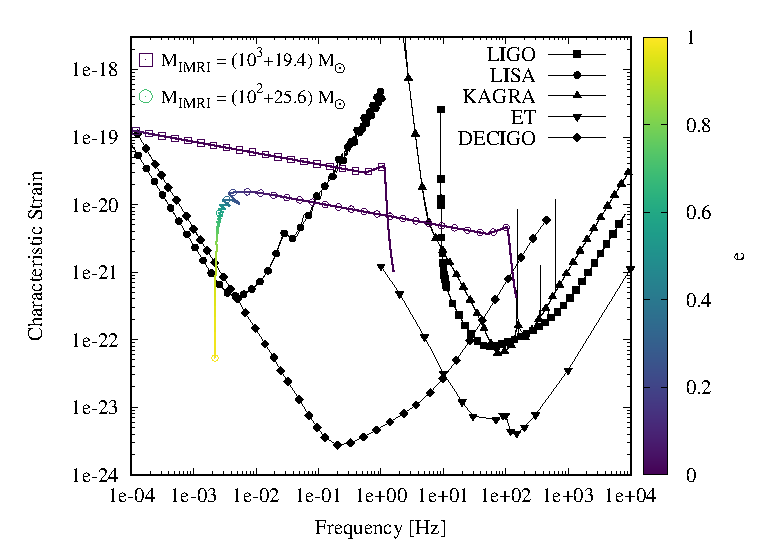
\includegraphics[width=8cm]{example_signal}\\
\caption{Strain calculated for the dominant frequency for two different models, assuming an infinite observational time. We overlap the simulated data with sensitivity curves from several GW observatories.}
\label{F12}
\end{figure}

\section{Conclusions}

\begin{itemize}
\item {\bf Make your point!}
\end{itemize}

\section*{Acknowledgements}

Sonderforschungsbereich SFB 881 "The Milky Way System" (subproject Z2) of the German Research Foundation (DFG) for the financial support provided. This work benefited of financial support from the Alexander von Humboldt Foundation, which granted MAS research program ``The evolution of black holes from stellar to galactic scales''. 
This work benefited from support by the ISSI (Bern), through its Intern. Team prog. ref. no. 393 {\it The Evolution of Rich Stellar Populations \& BH Binaries} (2017-18).


\footnotesize{
\bibliographystyle{mn2e}
\bibliography{ASetal2015}
}



\end{document}